\documentclass[border=5pt]{standalone}

\usepackage{tikz}

\begin{document}
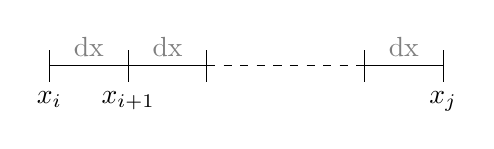
\begin{tikzpicture}[scale=1.0]
    \draw (0,-0.2) node [below] {$x_i$} -- (0,0.2);
    \draw (0,0) -- node [above, opacity=0.5] {dx} (1,0);

    \draw (1,-0.2) node [below] {$x_{i+1}$} -- (1,0.2) ;
    \draw (1,0) -- node [above, opacity=0.5] {dx} (2,0);

    \draw (2,-0.2) -- (2,0.2) ;
    \draw [dashed] (2,0) -- (4,0);

    \draw (4,-0.2) -- (4,0.2) ;
    \draw (4,0) -- node [above, opacity=0.5] {dx} (5,0);

    \draw (5,-0.2) node [below] {$x_{j}$} -- (5,0.2) ;
\end{tikzpicture}
\end{document}
